\documentclass[tikz,border=6pt]{standalone}
\usepackage[T1]{fontenc}
\usepackage[utf8]{inputenc}
\usepackage{pgfplots}
\usepgfplotslibrary{groupplots}
\usetikzlibrary{calc}
\pgfplotsset{compat=1.18}
\begin{document}
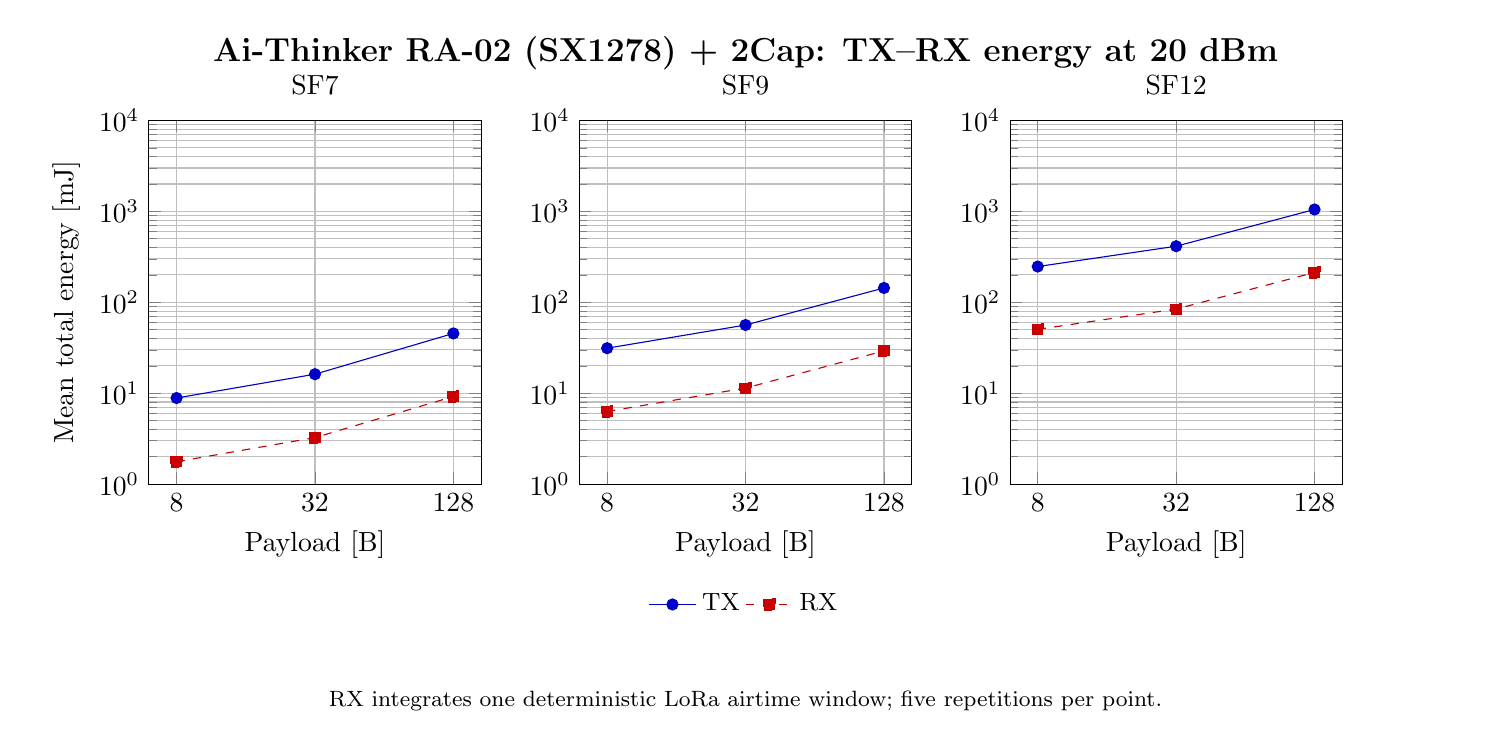
\begin{tikzpicture}
\begin{groupplot}[/pgf/number format/use comma, group style={group size=3 by 1, horizontal sep=1.25cm},
  width=5.8cm,height=6.2cm,xmode=log,log basis x=2,ymode=log,log basis y=10,ymin=1,ymax=10000,
  xtick={8,32,128},xticklabels={8,32,128},grid=both,xlabel={Payload [B]},
  legend style={draw=none,fill=none,font=\small,at={(0.5,-0.27)},anchor=north,legend columns=-1}]
% TX--RX energy
\nextgroupplot[title={SF7},ylabel={Mean total energy [mJ]}]
\addplot+[blue!75!black,solid,mark=*,error bars/.cd,y dir=both,y explicit] coordinates {(8,8.84459217) +- (0,0.0628122301) (32,16.1710185) +- (0,0.0760864794) (128,45.4043796) +- (0,0.234788619)};
\addplot+[red!75!black,dashed,mark=square*,error bars/.cd,y dir=both,y explicit] coordinates {(8,1.76122131) +- (0,0.00106864943) (32,3.24450476) +- (0,0.0035939822) (128,9.18337658) +- (0,0.0135579852)};
\nextgroupplot[title={SF9}]
\addplot+[blue!75!black,solid,mark=*,error bars/.cd,y dir=both,y explicit] coordinates {(8,31.2249375) +- (0,0.171757926) (32,56.2012148) +- (0,0.361300725) (128,143.588993) +- (0,0.663372236)};
\addlegendentry{TX}
\addplot+[red!75!black,dashed,mark=square*,error bars/.cd,y dir=both,y explicit] coordinates {(8,6.28297325) +- (0,0.00817412703) (32,11.3743267) +- (0,0.0109526015) (128,29.1720476) +- (0,0.056280913)};
\addlegendentry{RX}
\nextgroupplot[title={SF12}]
\addplot+[blue!75!black,solid,mark=*,error bars/.cd,y dir=both,y explicit] coordinates {(8,246.9808) +- (0,0.355324712) (32,413.462779) +- (0,1.3359441) (128,1048.34669) +- (0,1.85065565)};
\addplot+[red!75!black,dashed,mark=square*,error bars/.cd,y dir=both,y explicit] coordinates {(8,50.3459976) +- (0,0.0576104545) (32,84.1791207) +- (0,0.0466855073) (128,212.80557) +- (0,0.137079869)};
\end{groupplot}
\node[font=\bfseries\large] at ($(group c2r1.north)+(0,0.85cm)$) {Ai-Thinker RA-02 (SX1278) + 2Cap: TX--RX energy at 20 dBm};
\node[font=\footnotesize,align=center,text width=18cm] at ($(group c2r1.south)+(0,-2.75cm)$) {RX integrates one deterministic LoRa airtime window; five repetitions per point.};
\end{tikzpicture}
\end{document}
